\section{Classical Modular Forms}


\subsection{These are pretty cool!}

\begin{frame} \frametitle{Classical modular forms -- Definition 1}
  Modular forms are analytic functions on the complex upper half plane which have important number theoretical properties. \pause
  \begin{definition}
    A (classical) modular form $f$ of weight $k \in \NNO$ for the group $\SL[2]{\ZZ}$ is a function on the complex upper half plane $\HH = \setst{z \in \CC}{\Im{z} > 0}$ satisfying the following properties: \pause
    \begin{itemize}
      \item $f$ is complex analytic on $\HH$\pause,
      \item $f\parens{\frac{az+b}{cz+d}} = (cz+d)^{k} f(z)$ for all $a,b,c,d \in \ZZ$ such that $ad-bc = 1$\pause, and
      \item $\abs{f(z)}$ is bounded as $\Im{z} \to +\infty$.\pause \hfill \emph{(holomorphic at infinity)}
    \end{itemize}
  \end{definition}

  The second condition can be written as $f(\gamma z) = j(\gamma,z)^{-k} f(z)$ for all $\gamma = \parens{\begin{smallmatrix} a & b \\ c & d \end{smallmatrix}} \in \SL[2]{\ZZ}$, with \emph{factor of automorphy} $j(\gamma,z) = cz+d$.
\end{frame}


\begin{frame} \frametitle{Classical modular forms -- Definition 1}
  Here the group $\SL[2]{\ZZ}$ acts on $\HH$ from the left by the fractional linear transformation $z \xmapsto{\gamma} \frac{az+b}{cz+d}$, which is closely related to matrix multiplication on the left:
  \[ \begin{pmatrix} a & b \\ c & d \end{pmatrix} \begin{pmatrix} z \\ 1 \end{pmatrix} = \begin{pmatrix} az+b \\ cz+d \end{pmatrix} = \frac{1}{cz+d} \begin{pmatrix} \frac{az+b}{cz+d} \\ 1 \end{pmatrix}. \]
  \pause
  The left action of $\SL[2]{\ZZ}$ on $\HH$ translates into a right action on the functions $f : \HH \to \CC$:
  \[ f|_\gamma : \HH \to \CC, \quad z \mapsto j(\gamma,z)^{-k} f(\gamma z) = (cz+d)^{-k} f\parens{\frac{az+b}{cz+d}}. \]
  \pause
  The transformation condition in the previous definition can then be restated more simply: \pause
  \[ f|_\gamma(z) = f(z) \lsptext{for all} \gamma \in \SL[2]{\ZZ}. \]
\end{frame}


\begin{frame} \frametitle{Classical modular forms -- Definition 1}
  The first definition above is that of a modular form for the \emph{full} group $\SL[2]{\ZZ}$.
  More generally, for any $N \in \NN$ we can define a modular form for any \emph{congruence subgroup} $\Gamma \subseteq \SL[2]{\ZZ}$:
  \[ \Gamma \supseteq \Gamma(N) = \setst{\parens{\begin{smallmatrix} a & b \\ c & d \end{smallmatrix}} \in \SL[2]{\ZZ}}{\parens{\begin{smallmatrix} a & b \\ c & d \end{smallmatrix}} \equiv \parens{\begin{smallmatrix} 1 & 0 \\ 0 & 1 \end{smallmatrix}} \pmod{N}}: \pause \]
  \begin{definition}
    A modular form $f$ of weight $k$ for the congruence subgroup $\Gamma$ is a function $f : \HH \to \CC$ such that: \pause
    \begin{itemize}
      \item $f$ is complex analytic on $\HH$\pause,
      \item $f|_\gamma(z) = f(z)$ for all $\gamma \in \Gamma$\pause, and
      \item $\abs{f|_\gamma(z)}$ is bounded as $\Im{z} \to +\infty$ for all $\gamma \in \SL[2]{\ZZ}$. \pause \hfill \emph{(holomorphic at the cusps)}
    \end{itemize}
  \end{definition} \pause

  % Note that if $\Gamma = \Gamma(1) = \SL[2]{\ZZ}$, we get a modular form for the full group $\SL[2]{\ZZ}$.
\end{frame}


\subsection{A function on lattices?}

\begin{frame} \frametitle{Classical modular forms -- Definition 2}
  An alternative way to define a modular form is as a function on the space $\LL$ of lattices of rank $2$\pause; here a lattice (of rank $2$) is a free rank-$2$ additive subgroup $\Lambda = a\ZZ +b\ZZ \subset \CC$:\pause

  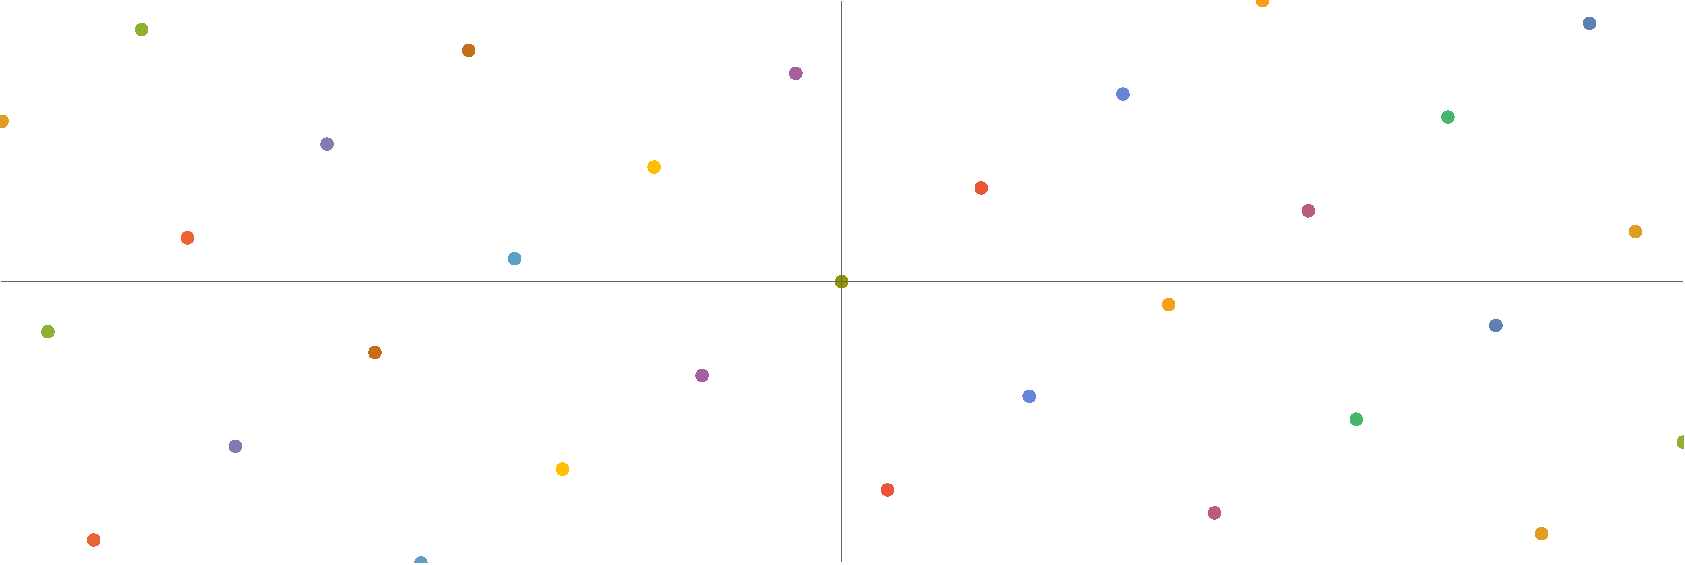
\includegraphics[width = \textwidth]{lattice.pdf}
\end{frame}


\begin{frame} \frametitle{Classical modular forms -- Definition 2}
  \begin{definition}
    A modular form $f$ of weight $k$ for $\SL[2]{\ZZ}$ is a function $f : \LL \to \CC$ such that:
    \begin{itemize}
      \item $f$ is analytic\pause, \hfill (?) \pause
      \item $f$ is homogeneous of degree $-k$: \pause $f(r\Lambda) = r^{-k} f(\Lambda)$ for all $r \in \CC^\times$ and $\Lambda \in \LL$\pause, and
      \item $\abs{f(\Lambda)}$ is bounded as long as the smallest element of $\Lambda$ is bounded away from $0$.\pause
    \end{itemize}
  \end{definition}

  If $f$ is a modular form in this lattice sense, then $\bar{f}(z) = f(z\ZZ+\ZZ)$ is a modular form in the complex-variable sense.
  In fact, the converse is also true, so that these two definitions are equivalent. \pause

  To define a modular form for the congruence subgroup $\Gamma(N)$ as a function of lattices we actually define it as a homogeneous function $f(\Lambda,\alpha)$ of a lattice $\Lambda$ together with a \emph{level structure} $\alpha : N^{-1}\Lambda/\Lambda \ionto (N^{-1}/\ZZ)^2$.
\end{frame}